\chapter{Docente}
<<<<<<< HEAD
\section{Registrar Programa Sintético}
Para registrar un Programa Sintético correspondiente a una Unidad de Aprendizaje, primero se da click en el \IUbutton{Ver Tareas} del menú lateral izquierdo.

\begin{figure}[!hbtp]
    \centering
    \includegraphics[width=0.4\linewidth]{images/SP6/VerTareas.png}
    \caption{Botón Ver Tareas} 
\end{figure}

Y la siguiente pantalla es desplegada:

\begin{figure}[H]
    \centering
    \hypertarget{RegLUA}{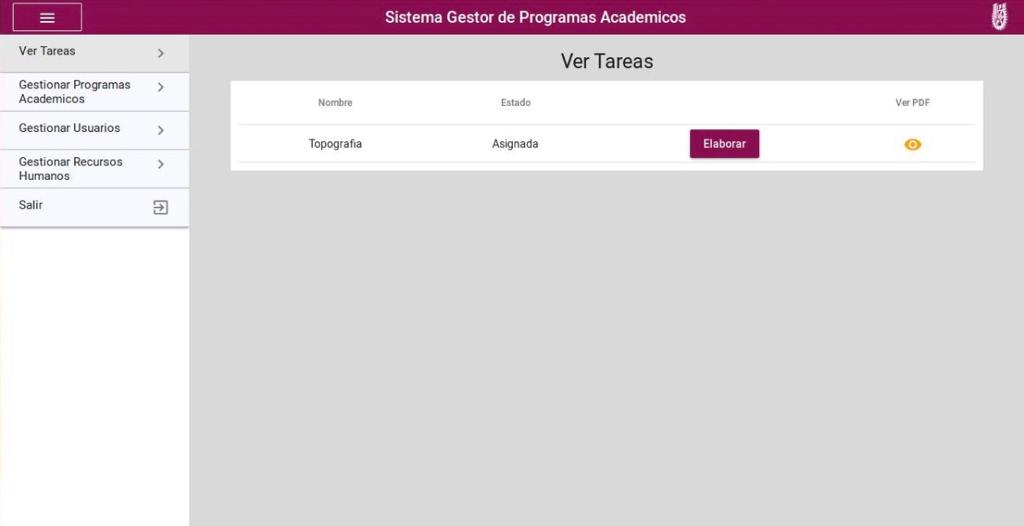
\includegraphics[width=0.7\linewidth]{images/SP6/PSListado.jpeg}}
    \caption{Pantalla Listado Unidades de Aprendizaje} 
\end{figure}

En la pantalla anterior se muestra un listado de las Unidades de Aprendizaje asignadas al Docente.

Para registrar un Programa Sintético correspondiente a una Unidad de Aprendizaje, el Docente da click sobre \IUbutton{Elaborar} y se muestra la pantalla:


\begin{figure}[H]
    \centering
    \hypertarget{RegPS}{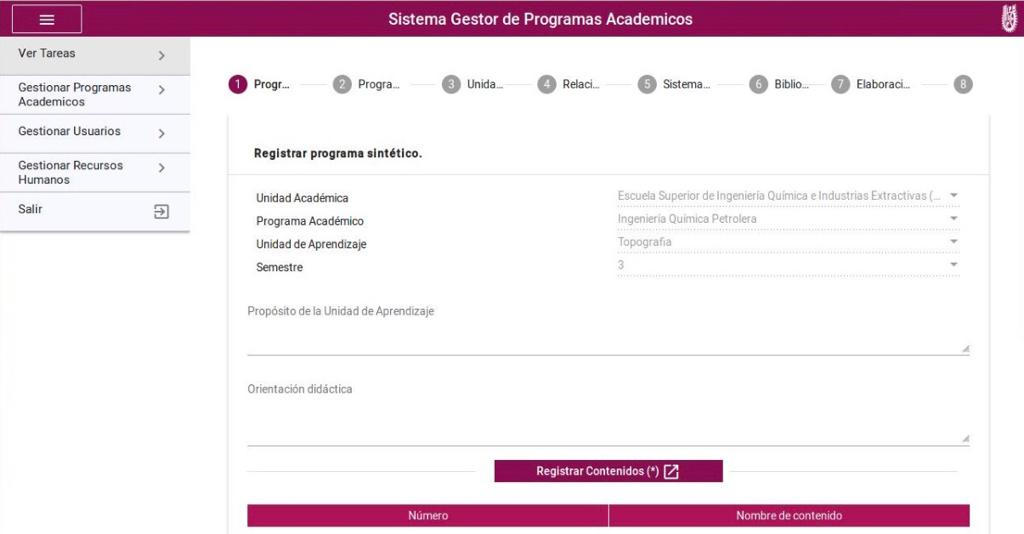
\includegraphics[width=0.7\linewidth]{images/SP6/PSinicio.jpeg}}
    
\includegraphics[width=0.7\linewidth]{images/SP6/PSinicio2.jpeg}
    \caption{Pantalla para Registrar Programa Sintético}
\end{figure}

Los campos desplegados en el formulario deberan ser llenados por el Docente.

Si el Docente desea:

\begin{itemize}
    \item Registrar Contenidos. El Docente debe dar click sobre el botón \IUbutton{Registrar Contenidos(*)}. Posteriormente consulte \hyperlink{RegC}{Registrar Contenido}
    \item Registrar Evaluación y Acreditación. El Docente debe dar click sobre el botón \IUbutton{Registrar Evaluación y Acreditación(*)}. Posteriormente consulte \hyperlink{RegEyA}{Registrar Evaluación y Acreditación}
\end{itemize}


Para concluir el registro. Revisar \hyperlink{GuardarFinalizar}{Guardar y/o Finalizar}
Si hay errores checar \hyperlink{Errores}{Posibles Errores}

\pagebreak
\hypertarget{RegC}{\subsection{Registrar Contenido}}

Para registrar un Contenido correspondiente a un Programa Sintético, se debe acceder por medio del botón \IUbutton{Registrar Contenidos(*)} de la pantalla \hyperlink{RegistrarPS}{Registrar Programa Sintético}. Posteriormente se muestra el siguiente formulario: 

\begin{figure}[H]
    \centering
    \hypertarget{RegC}{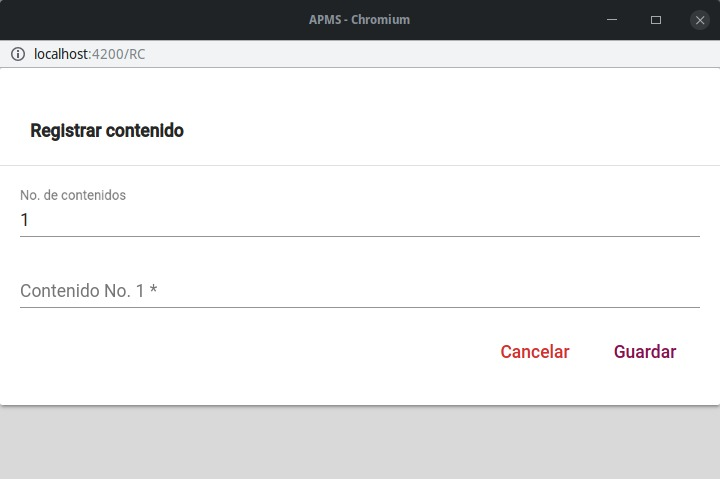
\includegraphics[width=0.5\linewidth]{images/SP6/11.jpeg}}
    \caption{Pantalla para Registrar Contenido}
\end{figure}

Para concluir el registro. Revisar \hyperlink{AceptarCancelar}{Aceptar y/o Cancelar}
Si hay errores checar

\hyperlink{Errores}{Posibles Errores}

\pagebreak
\hypertarget{RegEyA}{\subsection{Registrar Evaluación y Acreditación}}

Para registrar la Evaluación y Acreditación correspondiente a un Programa Sintético, se debe acceder por medio del botón \IUbutton{Evaluación y Acreditación(*)} de la pantalla \hyperlink{RegistrarPS}{Registrar Programa Sintético}. Posteriormente se muestra el siguiente formulario: 


\begin{figure}[H]
    \centering
    \hypertarget{RegEyA}{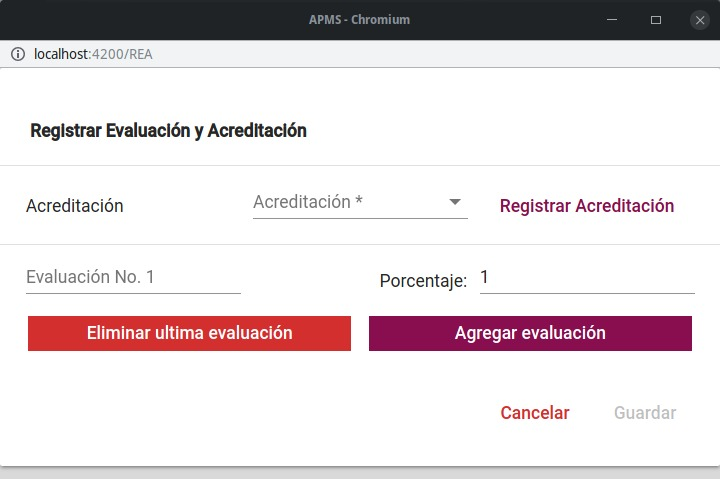
\includegraphics[width=0.5\linewidth]{images/SP6/8.jpeg}}
    \caption{Pantalla para Registrar Evaluación y Acreditación}
\end{figure}

Primeramente, el Docente debe seleccionar el tipo de Acreditación. En caso de no estar registrado debe dar click en el botón \IUbutton{Registrar Acreditación}(Consulte \hyperlink{RegA}{Registrar Acreditación}).

Posteriormente, se llena el campo de evaluación con el nombre y el porcentaje asignado. De ser necesario un nuevo tipo de evaluación, el Docente debe hacer click en el botón:

\begin{figure}[!h]
    \centering
    
\includegraphics[width=0.3\linewidth]{images/SP6/BotonEval.jpeg}
    \caption{Botón Agregar Evaluación} 
\end{figure}

Y se desplegara un nuevo campo para el nombre de la evaluación y un nuevo campo para el procentaje de dicha evaluación.

Si el Docente desea eliminar la ultima evaluación agregada deberá dar click al botón: 


\begin{figure}[H]
    \centering
    
\includegraphics[width=0.3\linewidth]{images/SP6/BotonEliEval.jpeg}
    \caption{Botón Eliminar Evaluación} 
\end{figure}

En caso de que los porcentajes de evaluación y acreditación no sumen 100\%, se muestra el mensaje:


\begin{figure}[H]
    \centering
    \hypertarget{XXX}{
\includegraphics[width=0.5\linewidth]{images/SP6/ErrorPorcentaje.jpeg}}
    \caption{Pantalla para Registrar Acreditación}
\end{figure}

De esta manera, el Docente debe corregir los datos para que sumen un total de 100\%.

Para concluir el registro. Revisar \hyperlink{AceptarCancelar}{Aceptar y/o Cancelar}
Si hay errores checar \hyperlink{Errores}{Posibles Errores}

\pagebreak
\hypertarget{RegA}{\subsection{Registrar Acreditación}}

Para registrar un nuevo tipo Acreditación correspondiente a un Programa Sintético, se debe acceder por medio del botón \IUbutton{Registrar Acreditación} de la pantalla \hyperlink{RegEyA}{Registrar Evaluación y Acreditación}. Posteriormente se muestra el siguiente formulario: 


\begin{figure}[H]
    \centering
    \hypertarget{RegA}{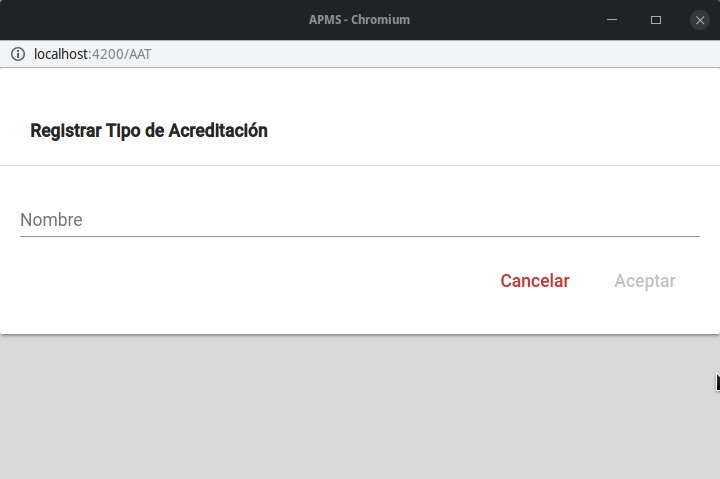
\includegraphics[width=0.5\linewidth]{images/SP6/9.jpeg}}
    \caption{Pantalla para Registrar Acreditación}
\end{figure}



Para concluir el registro. Revisar \hyperlink{AceptarCancelar}{Aceptar y/o Cancelar}
Si hay errores checar \hyperlink{Errores}{Posibles Errores}
\section{Registrar Programa en Extenso}

Para registrar el Programa en extenso correspondiente a una Unidad de Aprendizaje, primero se da click en en la pestaña \IUbutton{Ver Tareas}. y posteriormente en el botón \IUbutton{Programa en Extenso} y la siguiente pantalla será desplegada:

\begin{figure}[!hbtp]
    \centering
    \hypertarget{9}{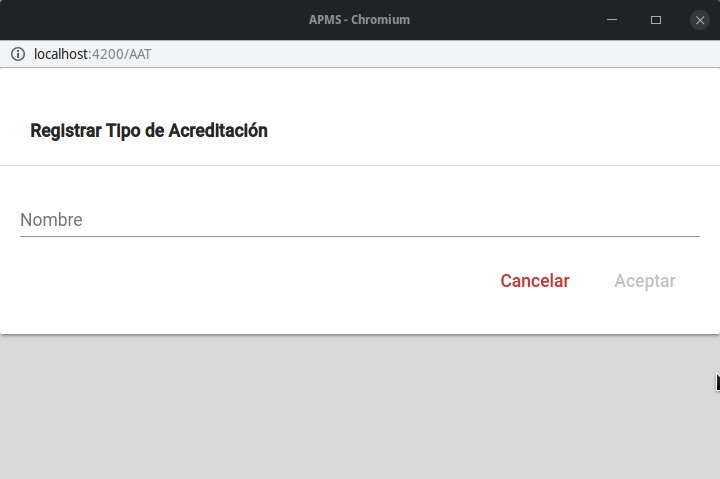
\includegraphics[width=0.5\linewidth]{images/SP6/9.jpeg}}
    \caption{Pantalla Registrar Programa en Extenso}
\end{figure}

Los campos desplegados en el formulario deberan ser llenados por el Docente.

Para concluir el registro. Revisar \hyperlink{GuardarFinalizar}{Guardar y Finalizar}

En caso de errores: 
    \begin{itemize}
        \item Revisar sección \hyperlink{Errores}{Posibles Errores}
    \end{itemize}

\section{Registrar Unidad Temática}

Para registrar una Unidad Temática  correspondiente a una Unidad de Aprendizaje, primero se da click en en la pestaña \IUbutton{Ver Tareas}. y posteriormente en el botón \IUbutton{Unidad Temática} y la siguiente pantalla será desplegada:

\hypertarget{RUT}{\begin{figure}[!hbtp]
    \centering
    \hypertarget{9}{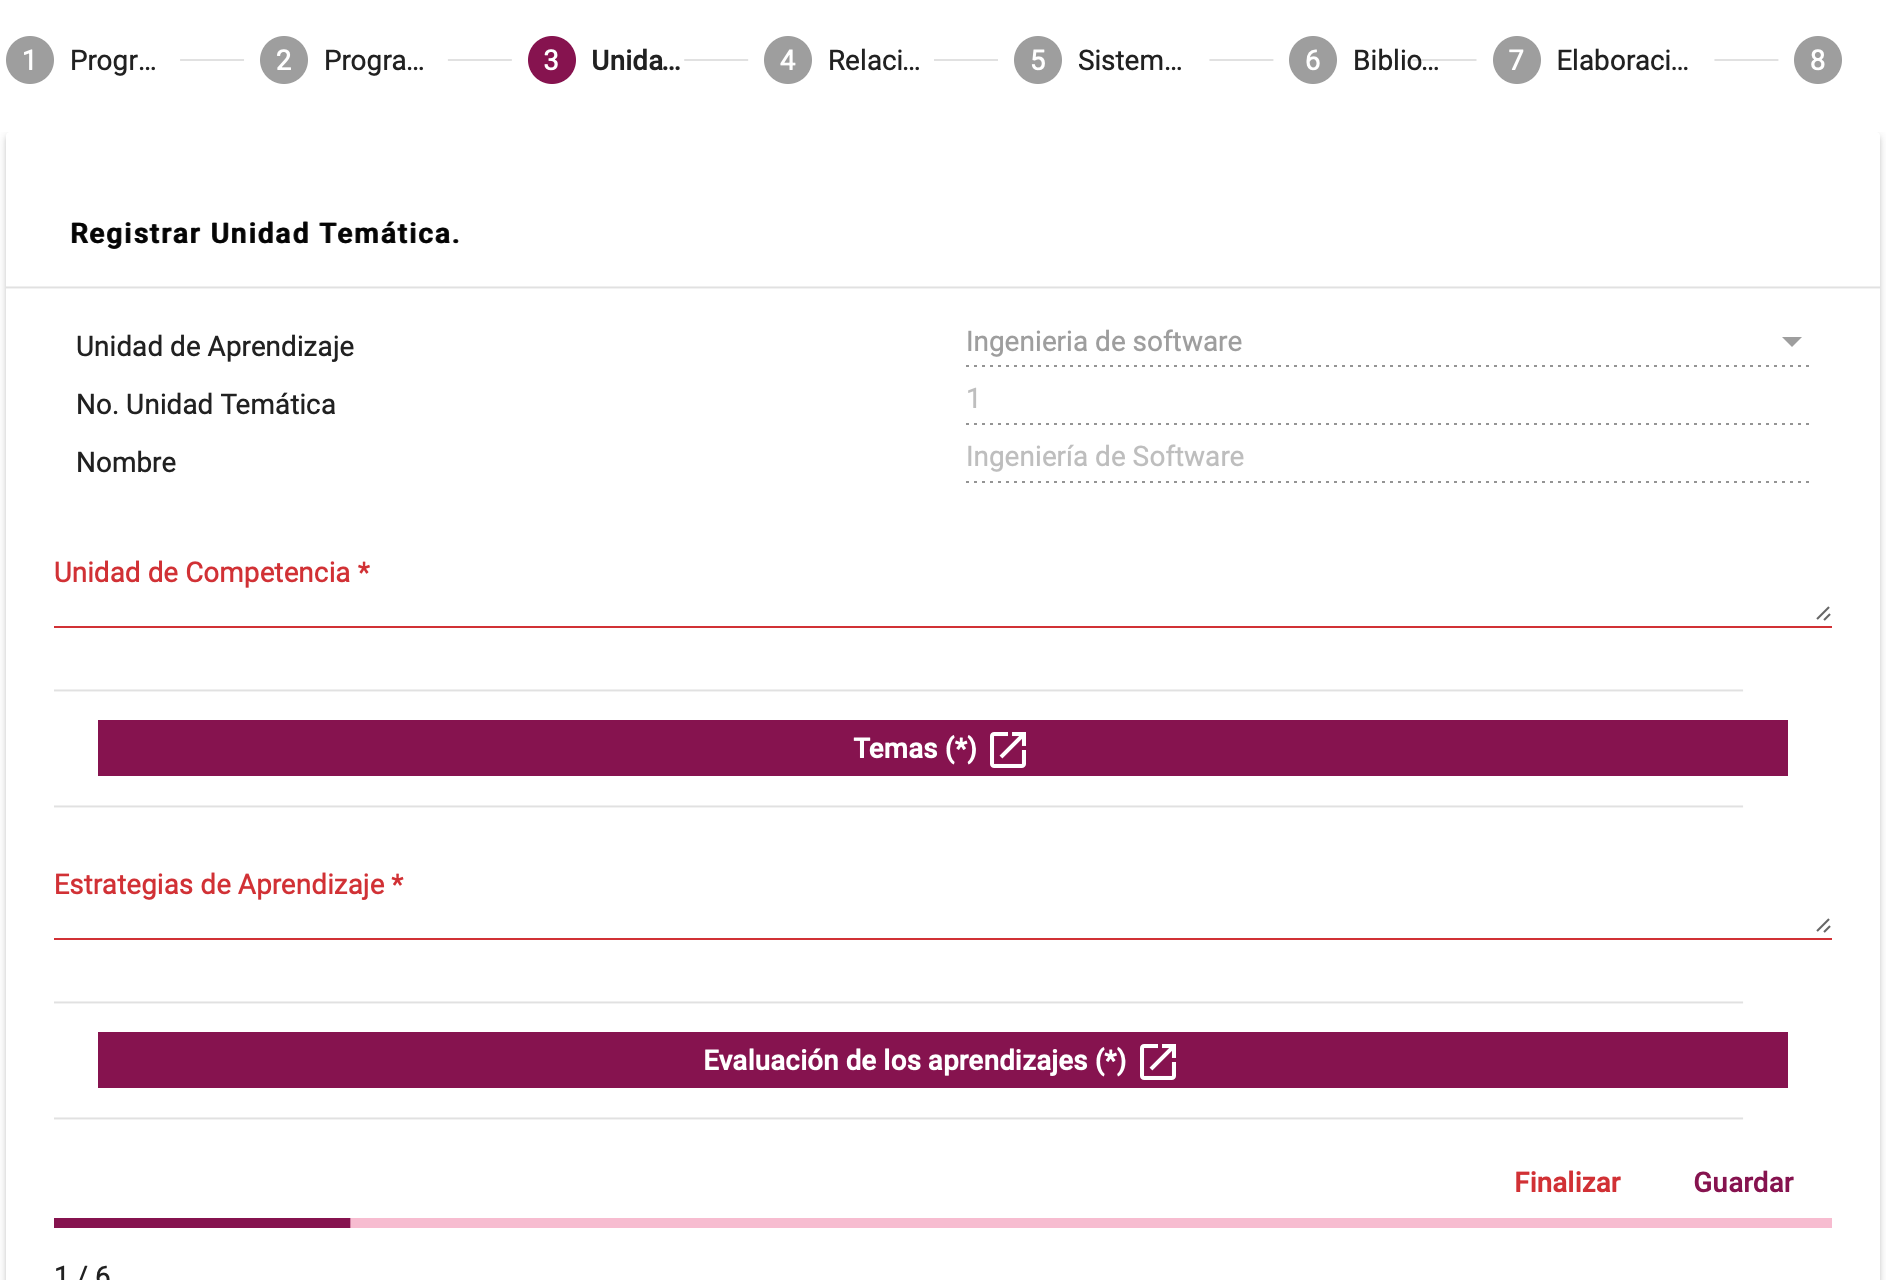
\includegraphics[width=0.5\linewidth]{images/SP6/RegistrarUT.png}}
    \caption{Pantalla para Registrar Unidad Temática}
\end{figure}
}


Los campos desplegados en el formulario deberan ser llenados por el Docente.

Si el Docente desea:

\begin{itemize}
    \item Registrar Temas. El Docente deberá dar click sobre el botón \IUbutton{Temas(*)}. Posteriormente consulte \hyperlink{RegistrarTema}{Registrar Tema}
    \item Registrar Evaluación de los Aprendizajes. El Docente deberá dar click sobre el botón \IUbutton{Evaluación de los Aprendizajes (*)}. Posteriormente consulte \hyperlink{RegistrarEvalAprend}{Registrar Evaluación y Acreditación}
\end{itemize}

Al llenar todos los datos correctamente, el Docente dará click en el botón:

Si hay errores checar \hyperlink{Errores}{Posibles Errores}

\pagebreak

\hypertarget{RegistrarTema}{\subsection{Registrar Tema}}
Para registrar un Tema correspondiente a una Unidad Temática, se debe acceder por medio del botón \IUbutton{Temas} de la pantalla \hyperlink{RUT}{Registrar Unidad Temática}. Posteriormente se mostrará la siguiente pantalla:

\hypertarget{RTema}{}
\begin{figure}[!hbtp]
    \centering
    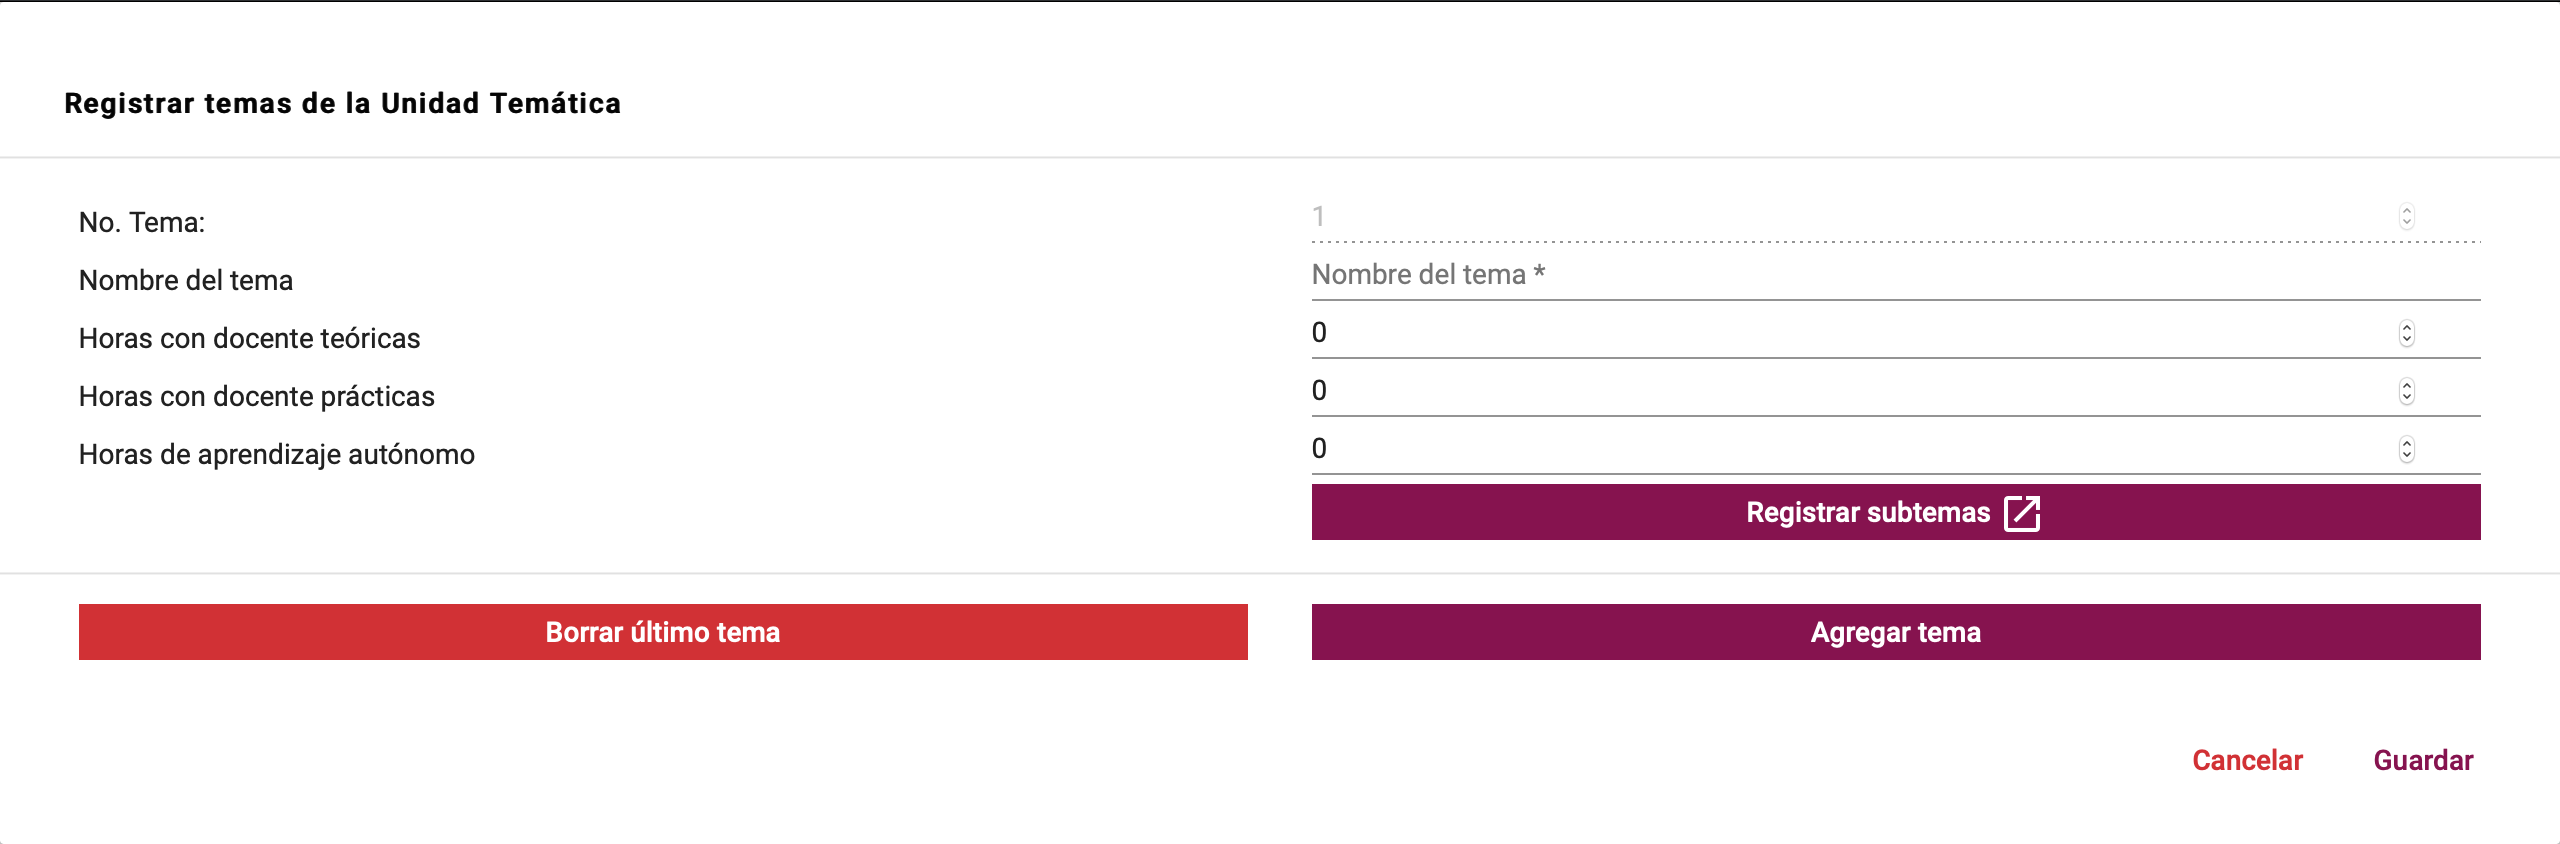
\includegraphics[width=0.7\linewidth]{images/SP6/RegistrarTema.png}
    \caption{Pantalla para Registrar Temas.} 
\end{figure}

Los campos desplegados en el formulario deberán ser llenados por el Docente.

Si el docente desea:
\begin{itemize}
    \item Registrar Subtema. Checar \hyperlink{RegistrarSubtema}{Registrar Subtema}.
    \item Agregar Tema. El docente da click al botón:
    \begin{figure}[!hbtp]
    \centering
    
\includegraphics[width=0.4\linewidth]{images/SP6/AgregarTema.png}
    \caption{Pantalla para Agregar Temas.} 
    \end{figure}
    Se agregará nuevos campos para un tema. Posteriormente el docente llena los nuevos campos.
    \item Eliminar Último Tema. El docente da click: al botón:
    \begin{figure}[!hbtp]
    \centering
    
\includegraphics[width=0.4\linewidth]{images/SP6/EliminarTema.png}
    \caption{Pantalla para Eliminar Temas.} 
    \end{figure}
    Se eliminará el último tema. Esto no aplica si solo hay un tema.
\end{itemize}

Para concluir el registro. Revisar \hyperlink{AceptarCancelar}{Aceptar o Cancelar}
Si hay errores checar \hyperlink{Errores}{Posibles Errores}

\pagebreak
\hypertarget{RegistrarSubtema}{\subsection{Registrar Subtema}}



Para registrar un Subtema correspondiente a Tema, se debe acceder por medio del botón \IUbutton{Subtema} de la pantalla \hyperlink{RTema}{Registrar Tema}. Posteriormente se mostrará la siguiente pantalla:

\begin{figure}[!hbtp]
    \centering
    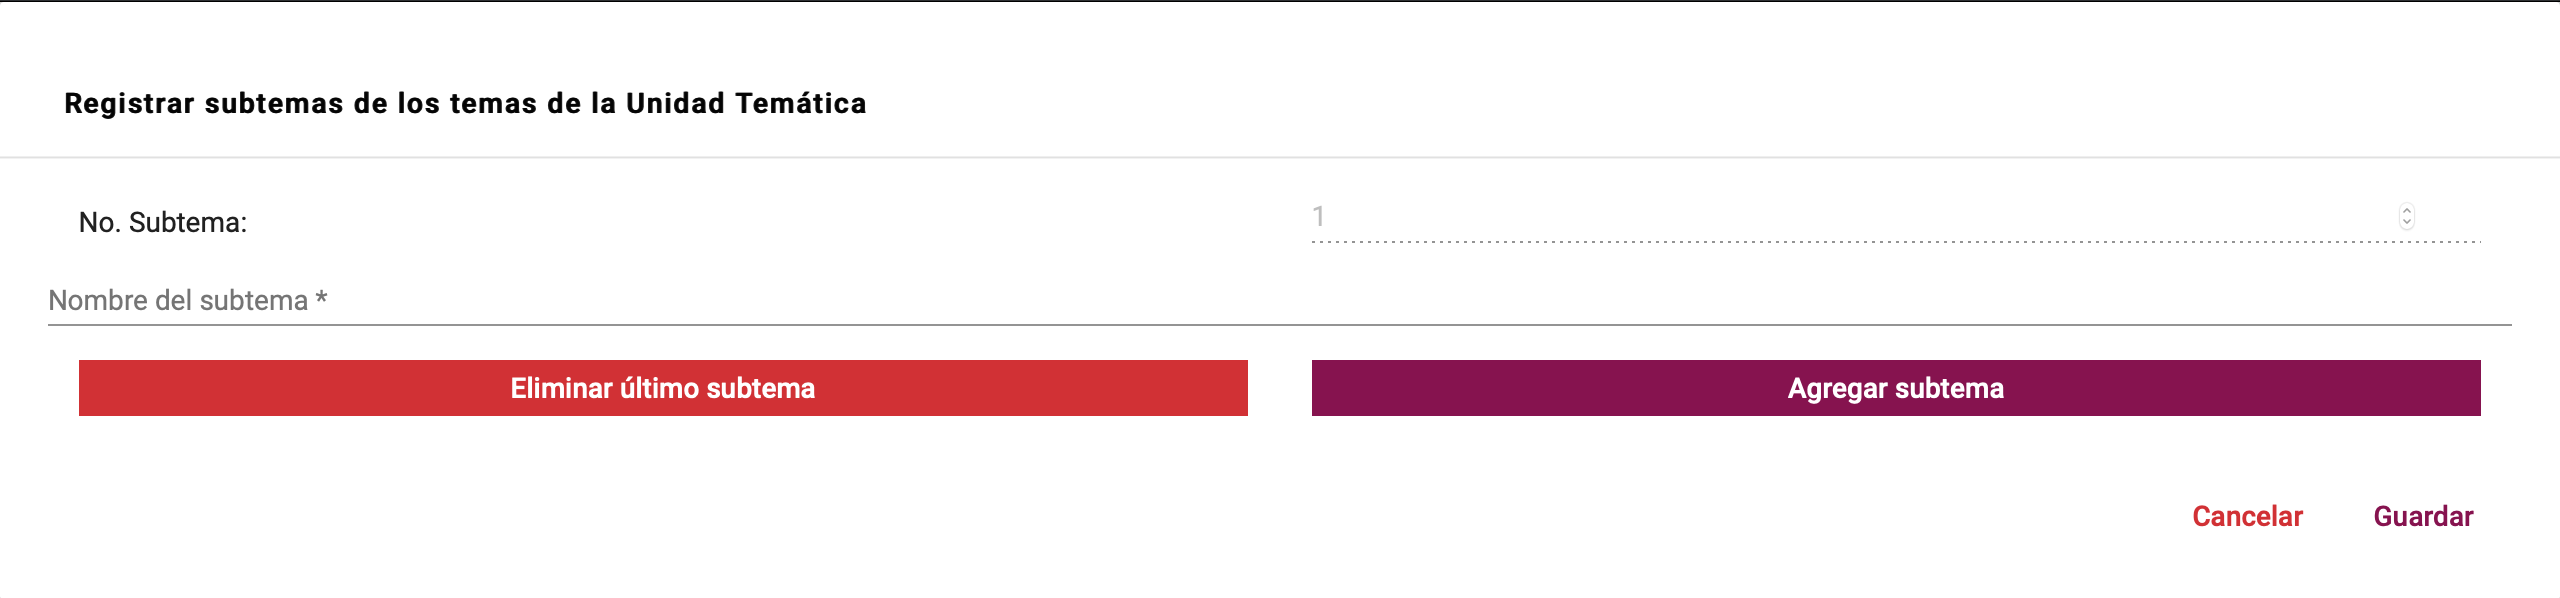
\includegraphics[width=0.7\linewidth]{images/SP6/RegistrarSubtema.png}
    \caption{Pantalla para Registrar Subtemas.} 
\end{figure}

Los campos desplegados en el formulario deberán ser llenados por el Docente.

Si el docente desea:
\begin{itemize}
    \item Agregar Subtema. El docente da click al botón:
    \begin{figure}[!hbtp]
    \centering
    
\includegraphics[width=0.4\linewidth]{images/SP6/AgregarSubtema.png}
    \caption{Pantalla para Agregar Subtemas.} 
    \end{figure}
    Se agregará nuevos campos para un tema. Posteriormente el docente llena los nuevos campos.
    \item Eliminar Último Subtema. El docente da click: al botón:
    \begin{figure}[!hbtp]
    \centering
    
\includegraphics[width=0.4\linewidth]{images/SP6/EliminarSubtema.png}
    \caption{Pantalla para Eliminar Temas.} 
    \end{figure}
    Se eliminará el último subtema. Esto no aplica si solo hay un subtema.
\end{itemize}

Para concluir el registro. Revisar \hyperlink{AceptarCancelar}{Aceptar o Cancelar}
Si hay errores checar \hyperlink{Errores}{Posibles Errores}

\pagebreak
\hypertarget{RegistrarEvalAprend}{\subsection{Registrar Evaluación de los Aprendizajes}}

Para registrar la Evaluación de los Aprendizajes correspondiente a una Unidad Temática, se debe acceder por medio del botón \IUbutton{Evaluación de los Aprendizajes} de la pantalla \hyperlink{RUT}{Registrar Unidad Temática}. Posteriormente se mostrará la siguiente pantalla:

\hypertarget{REvalApre}{}
\begin{figure}[!hbtp]
    \centering
    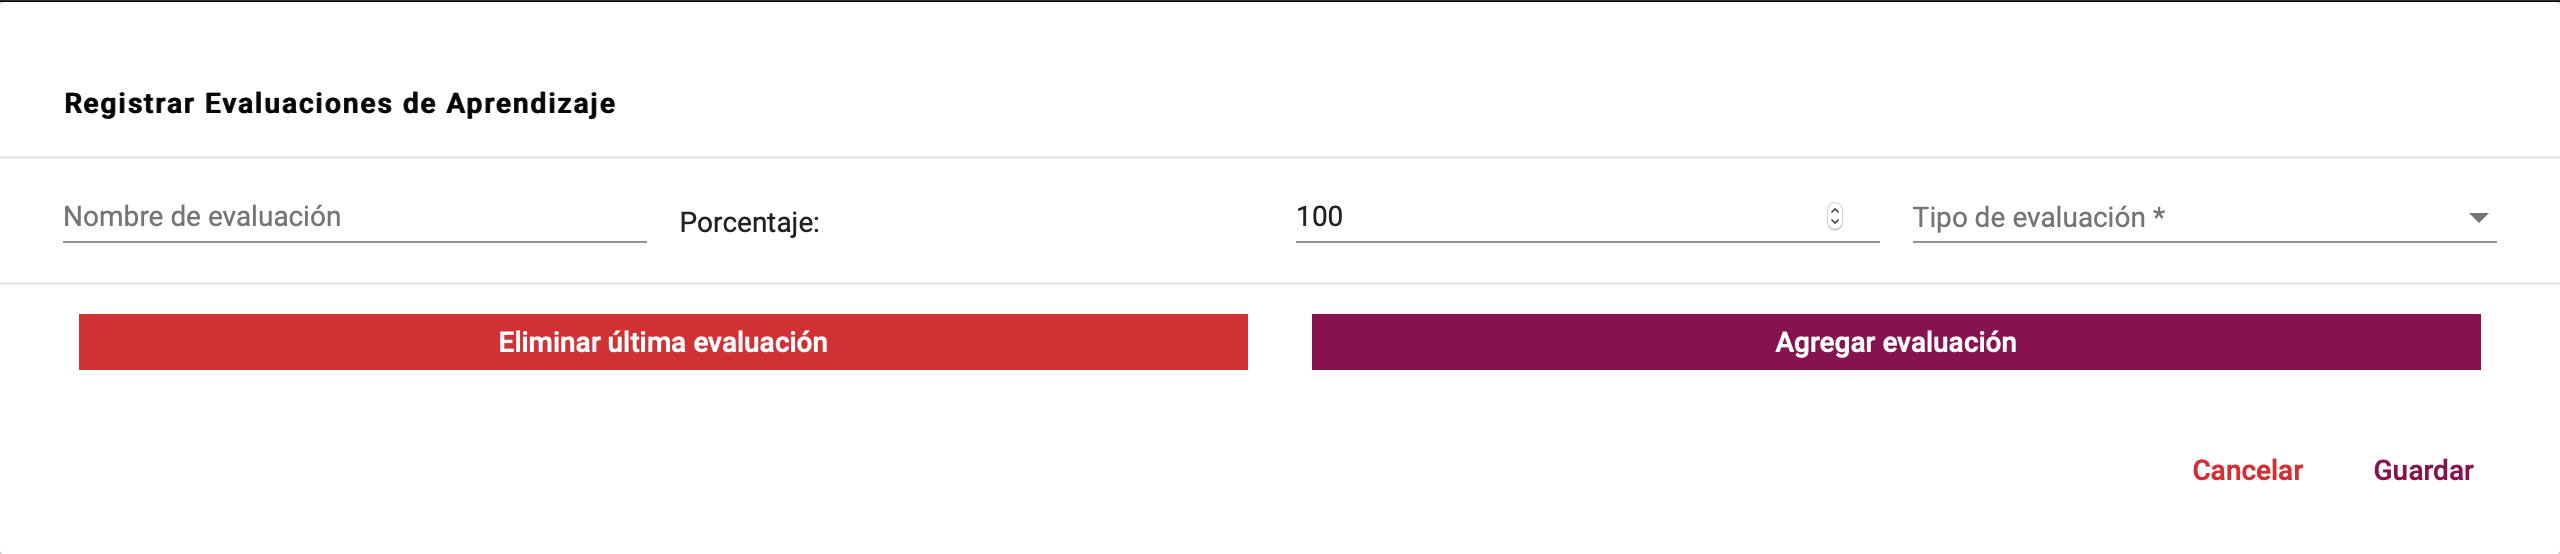
\includegraphics[width=0.7\linewidth]{images/SP6/RegistrarEvadeApren.png}
    \caption{Pantalla para Registrar Temas.} 
\end{figure}

Los campos desplegados en el formulario deberán ser llenados por el Docente.

Si el docente desea:
\begin{itemize}
    \item Agregar Evaluación. El docente da click al botón:
    \begin{figure}[!hbtp]
    \centering
    
\includegraphics[width=0.4\linewidth]{images/SP6/AgregarEval.png}
    \caption{Pantalla para Agregar Evaluación.} 
    \end{figure}
    Se agregará nuevos campos para una Evaluación. Posteriormente el docente llena los nuevos campos.
    \item Eliminar Última Evaluación. El docente da click: al botón:
    \begin{figure}[!hbtp]
    \centering
    
\includegraphics[width=0.4\linewidth]{images/SP6/ElimarEval.png}
    \caption{Pantalla para Eliminar Evaluación.} 
    \end{figure}
    Se eliminará el último Evaluación. Esto no aplica si solo hay una Evaluación.
\end{itemize}

Para concluir el registro. Revisar \hyperlink{GuardarFinalizar}{Guardar y Finalizar}
Si hay errores checar \hyperlink{Errores}{Posibles Errores}
\pagebreak


\pagebreak
\hypertarget{GuardarFinalizar}{\section{Guardar y/o Finalizar}}

Al llenar todos los datos correctamente, el Docente dará click en el botón:

\begin{figure}[!hbtp]
    \centering
    
\includegraphics[width=0.1\linewidth]{images/SP6/BotonFinalizar.jpeg}
    \caption{Botón Finalizar} 
\end{figure}

Se mostrara la siguiente pantalla:

\begin{figure}[!hbtp]
    \centering
    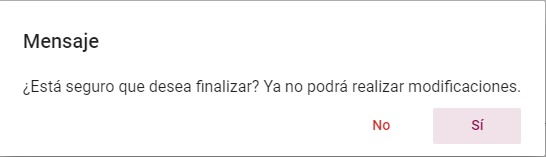
\includegraphics[width=0.6\linewidth]{images/SP6/DeseaRegistro.jpeg}
    \caption{¿Seguro que desea finalizar el registro?} 
\end{figure}

Al dar clic en \IUbutton{Aceptar} y si no se presentan errores se muestra el mensaje:


\begin{figure}[!hbtp]
    \centering
    
\includegraphics[width=0.4\linewidth]{images/SP6/MSGFINALIZAR.jpeg}
    \caption{Registro exitoso}
    \label{mensaje5}
\end{figure}

El sistema bloquea el formulario y se procede al siguiente formulario. 


Para continuar con el registro, usted tendrá que  dar click en \IUbutton{Cancelar}, el mensaje se cerrara y usted continuara 
en el formulario para terminar el registro.

Si el usuario requiere guardar el avance que ha ingresado: 

\begin{figure}[!hbtp]
    \centering
    
\includegraphics[width=0.1\linewidth]{images/SP6/BotonGuardar.jpeg}
    \caption{Botón Guardar} 
\end{figure}

El sistema guarda la información ingresada y muestra el mensaje: 

\begin{figure}[!hbtp]
    \centering
    
\includegraphics[width=0.4\linewidth]{images/SP6/MSGGUARDAR.jpeg}
    \caption{Botón Avances Guardados exitosamente.} 
\end{figure}



\pagebreak
\hypertarget{Errores}{\section{Posibles errores}}

    \begin{itemize}
        \item Problemas con la conexión o el sistema

        Si al momento de acceder a alguna  pantalla, aparece el siguiente mensaje:
                %Imagen MSG7 Y MSG25

        \begin{figure}[H]
            \centering
            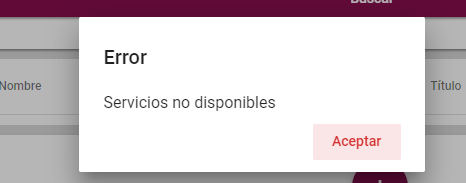
\includegraphics[width=0.4\linewidth]{images/SP6/MSGSN.png}
            \caption{Servicios no disponibles}
            \label{SND}

        \end{figure}

        Significa que existió un error de conexión o del sistema. Al dar clic en en botón ''Aceptar'', el sistema lo redireccionará a la pantalla anterior. Deberá esperar a que la página este disponible para  intentar acceder nuevamente.

        \item Campos vacíos al momento de ingresar el registro.

        Si usted deja en blanco algún campo o campos del formulario, y posteriormente dio clic en \IUbutton{Finalizar}, el sistema mostrará el siguiente mensaje debajo del campo o campos :

        \begin{figure}[H]
            \centering
            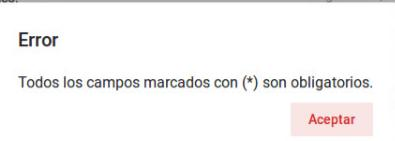
\includegraphics[width=0.4\linewidth]{images/SP6/Vacios.jpeg}
            \caption{Campos vacíos}
       \end{figure}

       Regresara al formulario, en donde usted deberá llenar el o los campos que dejo vacíos.

         \pagebreak
       \item Los campos ingresados no son válidos

       Si al momento de dar clic en \IUbutton{Finalizar} aparece el siguiente mensaje:
        \begin{figure}[H]
            \centering
            
\includegraphics[width=0.4\linewidth]{images/SP6/Invalida.jpeg}
            \caption{Campos incorrectos}
        \end{figure}

        Significa que la composición de los datos ingresados en el formulario no es la correcta.

    \end{itemize}

\pagebreak
\hypertarget{AceptarCancelar}{\section{Aceptar y/o Cancelar}}
El Docente deberá ingresar el nombre del tipo de Acreditación deseado. Finalmente dará click en el botón: 

\begin{figure}[!hbtp]
    \centering
    
\includegraphics[width=0.1\linewidth]{images/SP6/BotonAceptar.jpeg}
    \caption{Botón Aceptar} 
\end{figure}

Si el Docente desea cancelar el registro deberá dar click en el botón: 

\begin{figure}[!hbtp]
    \centering
    
\includegraphics[width=0.1\linewidth]{images/SP6/BotonCancelar.jpeg}
    \caption{Botón Cancelar} 
\end{figure}
=======
\section{Gestión de Programas Académicos}
\section{Registrar Programa Sintético}
Para registrar un Programa Sintético correspondiente a una Unidad de Aprendizaje, primero se da click en en la pestaña \IUbutton{Ver Tareas} y la siguiente pantalla será desplegada:

\begin{figure}[H]
    \centering
    \hypertarget{2}{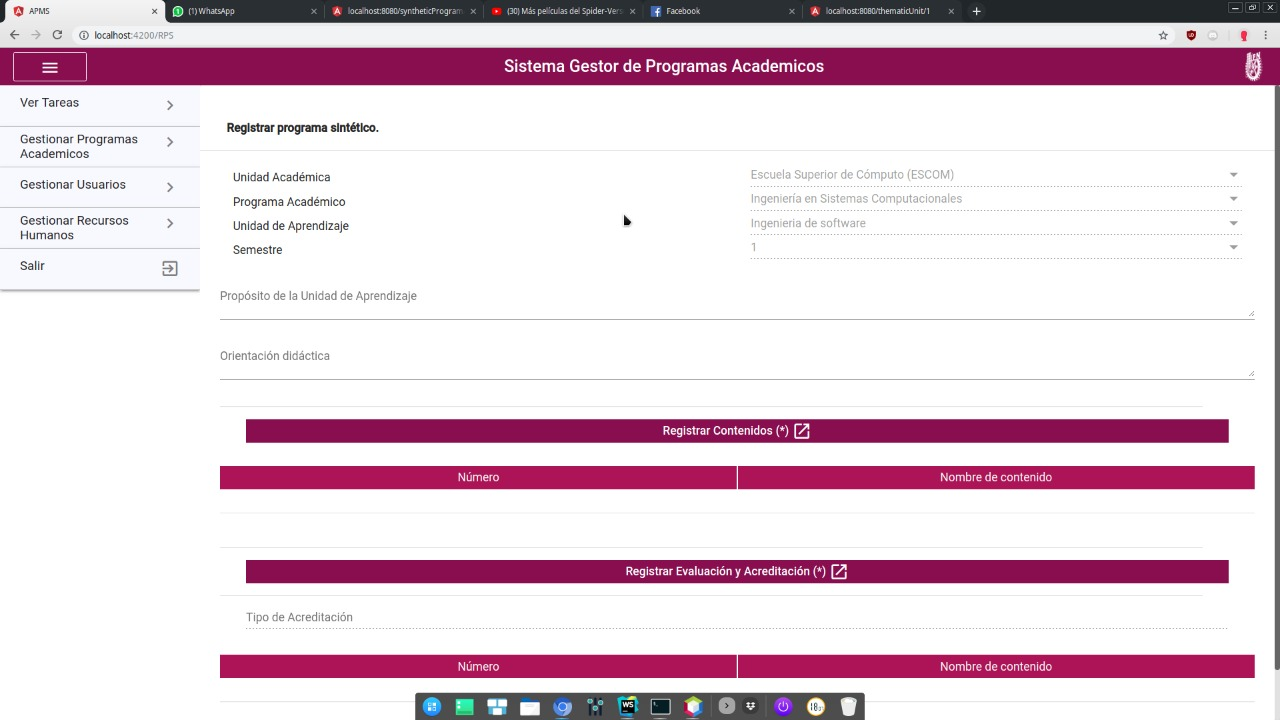
\includegraphics[width=0.5\linewidth]{images/SP6/1.jpeg}}
    \caption{Pantalla Listado Unidades de Aprendizaje}
\end{figure}

En la pantalla anterior se muestra un listado de las Unidades de Aprendizaje asignadas al Docente.

Para registrar una Programa Sintético correspondiente a una Unidad de Aprendizaje, el Docente debe dar click sobre el nombre de la Unidad de Aprendizaje y se mostrará la pantalla:

\pagebreak
\begin{figure}[H]
    \centering
    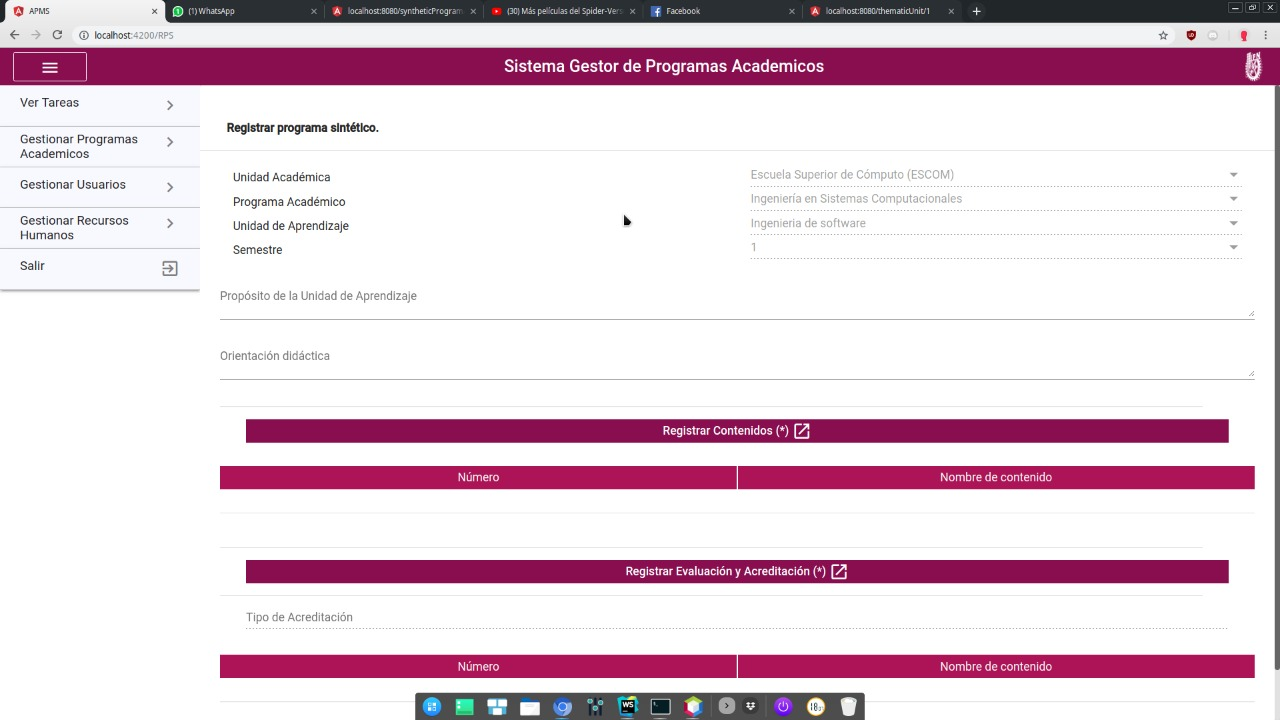
\includegraphics[width=0.5\linewidth]{images/SP6/1.jpeg}
    \caption{Pantalla para Registrar Programa Sintético}
\end{figure}

Los campos desplegados en el formulario deberan ser llenados por el Docente.

Si el Docente desea:

\begin{itemize}
    \item Registrar Contenidos. El Docente deberá dar click sobre el botón \IUbutton{Registrar Contenidos(*)}. Posteriormente consulte \hyperlink{Registrar Contenido}{Registrar Contenido}
    \item Registrar Evaluación y Acreditación. El Docente deberá dar click sobre el botón \IUbutton{Registrar Evaluación y Acreditación(*)}. Posteriormente consulte \hyperlink{REyA}{Registrar Evaluación y Acreditación}
\end{itemize}

Al llenar todos los datos correctamente, el Docente dará click en el botón:

\begin{figure}[H]
    \centering
    
\includegraphics[width=0.1\linewidth]{images/SP6/BotonFinalizar.jpeg}
    \caption{Botón Finalizar}
\end{figure}

Se mostrara la siguiente pantalla:
%%%%%%%%%%%%%%%%%%%%%%%% Corrección %%%%%%%%%%%%%%%%%%%%%%%%%%%%%
%%%%%%%%%%%%%%%%%%%%%%%%%%%%%%%%%%%%%%%%%%%%%%%%%%%%%%%%%%%%%%%
% \begin{figure}[H]
%     \centering
%     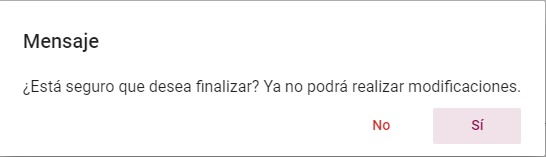
\includegraphics[width=0.1\linewidth]{images/SP6/DeseaRegistro.jpeg}
%     \caption{¿Seguro que desea finalizar el registro?}
% \end{figure}
%%%%%%%%%%%%%%%%%%%%%%%%%%%%%%%%%%%%%%%%%%%%%%%%%%%%%%%%%%%%%%%%
Al dar clic en \IUbutton{Aceptar} y si no se presentan errores se muestra el mensaje:


\begin{figure}[H]
    \centering
    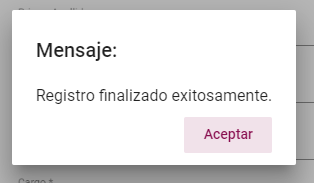
\includegraphics[width=0.4\linewidth]{images/SP6/MSG5.png}
    \caption{Registro exitoso}
    \label{mensaje5}
\end{figure}


El sistema bloquea el formulario y se procede al siguiente formulario. \hyperlink{RPE}{Registrar Programa en Extenso}


Para continuar con el registro, usted tendrá que  dar click en \IUbutton{Cancelar}, el mensaje se cerrara y usted continuara
en el formulario para terminar el registro.

\pagebreak
Si el usuario requiere guardar el avance que ha ingresado:

\begin{figure}[H]
    \centering
    
\includegraphics[width=0.1\linewidth]{images/SP6/BotonGuardar.jpeg}
    \caption{Botón Guardar}
\end{figure}

El sistema guarda la información ingresada y muestra el mensaje:

\begin{figure}[H]
    \centering
    
\includegraphics[width=0.4\linewidth]{images/SP6/BotonAvance.jpeg}
    \caption{Botón Avances Guardados exitosamente.}
\end{figure}

\subsubsection{Posibles errores}

    \begin{itemize}
        \item Problemas con la conexión o el sistema

        Si al momento de acceder a la pantalla de \hyperlink{registrarPS}{\textit{Registrar Programa Sintético}} o al intentar registrar una Unidad de Aprendizaje, aparece el siguiente mensajes:
                %Imagen MSG7 Y MSG25

        \begin{figure}[H]
            \centering
            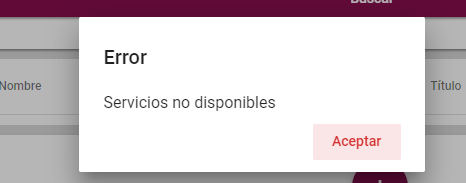
\includegraphics[width=0.4\linewidth]{images/SP6/MSGSN.png}
            \caption{Servicios no disponibles}
            \label{SND}

        \end{figure}

        Significa que existió un error de conexión o del sistema. Al dar clic en en botón ''Aceptar'', el sistema lo redireccionará a la pantalla de \hyperlink{verTareas}{\textit{Listado de Unidades de Aprendizaje}}. Deberá esperar a que la página este disponible para  intentar acceder nuevamente.

        \item Campos vacíos al momento de ingresar un Programa Sintético

        Si usted deja en blanco algún campo o campos del formulario, y posteriormente dio clic en \IUbutton{Finalizar}, el sistema mostrará el siguiente mensaje debajo del campo o campos :

       %  \begin{figure}[H]
       %      \centering
       %      
\includegraphics[width=0.1\linewidth]{images/SP6/MSG44.png}
       %      \caption{Campos vacíos}
       %      \label{mensaje44}
       % \end{figure}

       Regresara al formulario, en donde usted deberá llenar el o los campos que dejo vacíos.

       \item Los campos ingresados no son válidos

       Si al momento de dar clic en \IUbutton{Finalizar} aparece el siguiente mensaje:
          %Imagen MSG35
         % Imagen del MSG35
        % \begin{figure}[H]
        %     \centering
        %     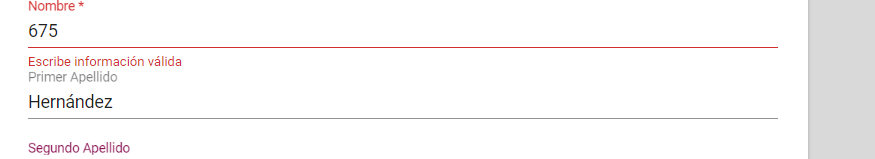
\includegraphics[width=0.1\linewidth]{images/SP6/MSG35.png}
        %     \caption{Campos incorrectos}
        %     \label{mensaje35}
        % \end{figure}

        Significa que la composición de los datos ingresados en el formulario no es la correcta. Tenga en cuenta lo siguiente:

        \begin{itemize}
            \item
            \item

        \end{itemize}

    \end{itemize}

\pagebreak
\hypertarget{Registrar Contenido}{\section{Registrar Contenido}}

Para registrar un Contenido correspondiente a un Programa Sintético, se debe acceder por medio del botón \IUbutton{Registrar Contenidos(*)} de la pantalla \hyperlink{RegistrarPS}{Registrar Programa Sintético}. Posteriormente se mostrará el siguiente formulario:


\begin{figure}[H]
    \centering
    \hypertarget{RegistrarContenido}{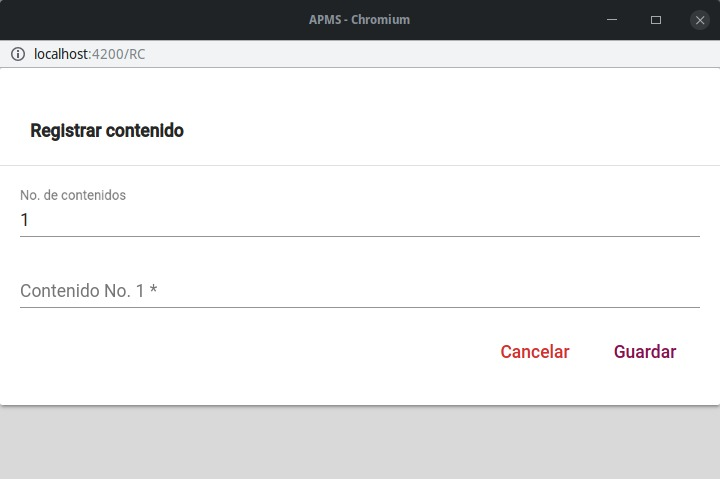
\includegraphics[width=0.5\linewidth]{images/SP6/11.jpeg}}
    \caption{Pantalla para Registrar Contenido}
\end{figure}

Al terminar, ya que los datos son llenados, el Docente dará click en el botón:

\begin{figure}[H]
    \centering
    
\includegraphics[width=0.1\linewidth]{images/SP6/BotonGuardar.jpeg}
    \caption{Botón Guardar}
\end{figure}

Si el Docente desea cancelar el registro deberá dar click en el botón:

\begin{figure}[H]
    \centering
    
\includegraphics[width=0.1\linewidth]{images/SP6/BotonCancelar.jpeg}
    \caption{Botón Cancelar}
\end{figure}
\pagebreak
\hypertarget{REyA}{\section{Registrar Evaluación y Acreditación}}


Para registrar la Evaluación y Acreditación correspondiente a un Programa Sintético, se debe acceder por medio del botón \IUbutton{Evaluación y Acreditación(*)} de la pantalla \hyperlink{RegistrarPS}{Registrar Programa Sintético}. Posteriormente se mostrará el siguiente formulario:


\begin{figure}[!h]
    \centering
    \hypertarget{RegistrarEC}{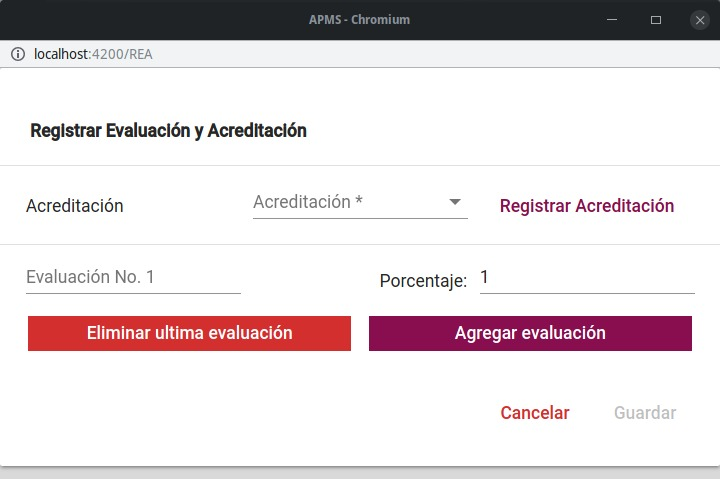
\includegraphics[width=0.5\linewidth]{images/SP6/8.jpeg}}
    \caption{Pantalla para Registrar Evaluación y Acreditación}
\end{figure}

Primeramente, el Docente deberá seleccionar el tipo de Acreditación. En caso de no estar registrado deberá dar click en el botón \IUbutton{Registrar Acreditación}(Consulte \hyperlink{RegAcre}{Registrar Acreditación}).

Posteriormente, se llenará el campo de evaluación con el nombre y el porcentaje asignado. De ser necesario un nuevo tipo de evaluación, el Docente deberá hacer click en el botón:

\begin{figure}[!h]
    \centering
    
\includegraphics[width=0.3\linewidth]{images/SP6/BotonEval.jpeg}
    \caption{Botón Agregar Evaluación}
\end{figure}

Y se desplegara un nuevo campo para el nombre de la evaluación y un nuevo campo para el procentaje de dicha evaluación.

Si el Docente desea eliminar la última evaluación agregada deberá dar click al botón:


\begin{figure}[!h]
    \centering
    
\includegraphics[width=0.3\linewidth]{images/SP6/BotonEliEval.jpeg}
    \caption{Botón Eliminar Evaluación}
\end{figure}


Al terminar, ya que los datos son llenados, el Docente dará click en el botón:

\begin{figure}[H]
    \centering
    
\includegraphics[width=0.1\linewidth]{images/SP6/BotonGuardar.jpeg}
    \caption{Botón Guardar}
\end{figure}

Si el Docente desea cancelar el registro deberá dar click en el botón:

\begin{figure}[H]
    \centering
    
\includegraphics[width=0.1\linewidth]{images/SP6/BotonCancelar.jpeg}
    \caption{Botón Cancelar}
\end{figure}


\pagebreak
\hypertarget{RegAcre}{\section{Registrar Acreditación}}


Para registrar la Evaluación y Acreditación correspondiente a un Programa Sintético, se debe acceder por medio del botón \IUbutton{Registrar Acreditación} de la pantalla \hyperlink{RegistrarEC}{Registrar Evaluación y Acreditación}. Posteriormente se mostrará el siguiente formulario:


\begin{figure}[!h]
    \centering
    \hypertarget{RegistrarAcreditacion}{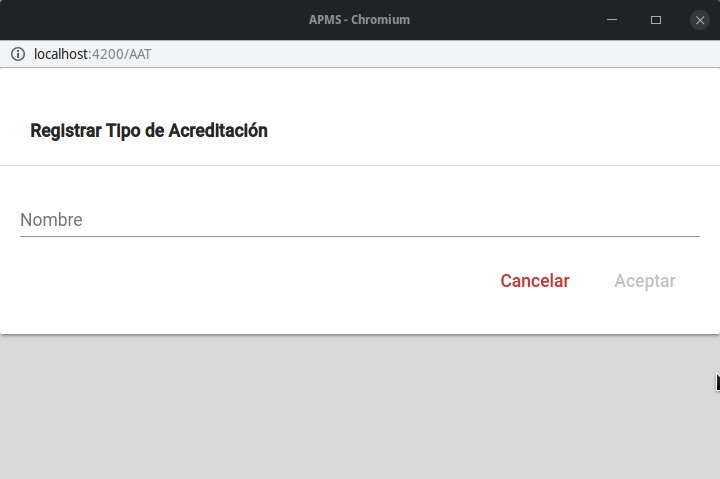
\includegraphics[width=0.5\linewidth]{images/SP6/9.jpeg}}
    \caption{Pantalla para Registrar Acreditación}
\end{figure}

El Docente deberá ingresar el nombre del tipo de Acreditación deseado. Finalmente dará click en el botón:

\begin{figure}[H]
    \centering
    \includegraphics[width=0.1\linewidth]{images/SP6/BotonAceptar.jpeg}
    \caption{Botón Aceptar}
\end{figure}

Si el Docente desea cancelar el registro deberá dar click en el botón:

\begin{figure}[H]
    \centering
    \includegraphics[width=0.1\linewidth]{images/SP6/BotonCancelar.jpeg}
    \caption{Botón Cancelar}
\end{figure}
\pagebreak
\hypertarget{RegPE}{\section{Registrar Programa en Extenso}}

Para registrar el Programa en extenso correspondiente a una Unidad de Aprendizaje, primero se da click en en la pestaña \IUbutton{Ver Tareas}. y posteriormente en el botón \IUbutton{Programa en Extenso} y la siguiente pantalla será desplegada:

\begin{figure}[!h]
    \centering
    \hypertarget{RegPE}{\includegraphics[width=0.5\linewidth]{images/SP6/9.jpeg}}
    \caption{Pantalla Registrar Programa en Extenso}
\end{figure}

Los campos desplegados en el formulario deberan ser llenados por el Docente.

Si el Docente desea:

\begin{itemize}
    \item Registrar Tiempos Asignados. El Docente deberá dar click sobre el botón \IUbutton{Registrar Tiempos Asignados(*)}. Posteriormente consulte \hyperlink{RegTA}{Registrar Tiempos Asignados}
\end{itemize}

Al llenar todos los datos correctamente, el Docente dará click en el botón:

\begin{figure}[H]
    \centering
    \includegraphics[width=0.1\linewidth]{images/SP6/BotonFinalizar.jpeg}
    \caption{Botón Finalizar}
\end{figure}

Se mostrara la siguiente pantalla:
%%%%%%%%%%%%%%%%%%%%%%%%%%%%%%%%%%%%%%%%%%%%%%%%%%%%%%%%%%%%%%
% \begin{figure}[H]
%     \centering
%     \includegraphics[width=0.1\linewidth]{images/SP6/DeseaRegistro.jpeg}
%     \caption{¿Seguro que desea finalizar el registro?}
% \end{figure}
%%%%%%%%%%%%%%%%%%%%%%%%%%%%%%%%%%%%%%%%%%%%%%%%%%%%%%%%%%%%%55
Al dar clic en \IUbutton{Aceptar} y si no se presentan errores se muestra el mensaje:


\begin{figure}[H]
    \centering
    \includegraphics[width=0.4\linewidth]{images/SP6/MSG5.png}
    \caption{Registro exitoso}
    \label{mensaje5}
\end{figure}


El sistema bloquea el formulario y se procede al siguiente formulario. \hyperlink{RegUT}{Registrar Unidad Temática}


Para continuar con el registro, usted tendrá que  dar click en \IUbutton{Cancelar}, el mensaje se cerrara y usted continuara
en el formulario para terminar el registro.

\pagebreak
Si el usuario requiere guardar el avance que ha ingresado:

\begin{figure}[H]
    \centering
    \includegraphics[width=0.1\linewidth]{images/SP6/BotonGuardar.jpeg}
    \caption{Botón Guardar}
\end{figure}

El sistema guarda la información ingresada y muestra el mensaje:

\begin{figure}[H]
    \centering
    \includegraphics[width=0.4\linewidth]{images/SP6/BotonAvance.jpeg}
    \caption{Botón Avances Guardados exitosamente.}
\end{figure}

\subsubsection{Posibles errores}

    \begin{itemize}
        \item Problemas con la conexión o el sistema

        Si al momento de acceder a la pantalla de \hyperlink{RegPE}{\textit{Registrar Programa en Extenso}} o al intentar registrar una Unidad de Aprendizaje, aparece el siguiente mensajes:
                %Imagen MSG7 Y MSG25

        \begin{figure}[H]
            \centering
            \includegraphics[width=0.4\linewidth]{images/SP6/MSGSN.png}
            \caption{Servicios no disponibles}
            \label{SND}

        \end{figure}

        Significa que existió un error de conexión o del sistema. Al dar clic en en botón ''Aceptar'', el sistema lo redireccionará a la pantalla de \hyperlink{verTareas}{\textit{Listado de Unidades de Aprendizaje}}. Deberá esperar a que la página este disponible para  intentar acceder nuevamente.

        \item Campos vacíos al momento de ingresar un Programa Sintético

        Si usted deja en blanco algún campo o campos del formulario, y posteriormente dio clic en \IUbutton{Finalizar}, el sistema mostrará el siguiente mensaje debajo del campo o campos :
%%%%%%%%%%%%%%%%%%%%%%%%%%%%%%%%%%%%%%%%%%%%%%%%%%%%%%%%%%%%%%%%%%%
       %  \begin{figure}[H]
       %      \centering
       %      \includegraphics[width=0.1\linewidth]{images/SP6/MSG44.png}
       %      \caption{Campos vacíos}
       %      \label{mensaje44}
       % \end{figure}
%%%%%%%%%%%%%%%%%%%%%%%%%%%%%%%%%%%%%%%%%%%%%%%%%%%%%%%%%%%%%%%%%%%%
       Regresara al formulario, en donde usted deberá llenar el o los campos que dejo vacíos.

       \item Los campos ingresados no son válidos

       Si al momento de dar clic en \IUbutton{Finalizar} aparece el siguiente mensaje:
          %Imagen MSG35
         % Imagen del MSG35
%%%%%%%%%%%%%%%%%%%%%%%%%%%%%%%%%%%%%%%%%%%%%%%%%%%%%%%%%%%%%%%%%%%%%%%%%%%%%
%         \begin{figure}[H]
%             \centering
%             \includegraphics[width=0.1\linewidth]{images/SP6/MSG35.png}
%             \caption{Campos incorrectos}
%             \label{mensaje35}
%         \end{figure}
%%%%%%%%%%%%%%%%%%%%%%%%%%%%%%%%%%%%%%%%%%%%%%%%%%%%%%%%%%%%%%%%%%%%%%%
        Significa que la composición de los datos ingresados en el formulario no es la correcta. Tenga en cuenta lo siguiente:

        \begin{itemize}
            \item
            \item

        \end{itemize}

    \end{itemize}

\pagebreak
\hypertarget{RegUT}{\section{Registrar Unidad Temática}}

Para registrar una Unidad Temática  correspondiente a una Unidad de Aprendizaje, primero se da click en en la pestaña \IUbutton{Ver Tareas}. y posteriormente en el botón \IUbutton{Unidad Temática} y la siguiente pantalla será desplegada:

\begin{figure}[!h]
    \centering
    \hypertarget{RegistrarUnidadTematica}{\includegraphics[width=0.5\linewidth]{images/SP6/9.jpeg}}
    \caption{Pantalla para Registrar Unidad Temática}
\end{figure}

Los campos desplegados en el formulario deberan ser llenados por el Docente.

Si el Docente desea:

\begin{itemize}
    \item Registrar Temas. El Docente deberá dar click sobre el botón \IUbutton{Temas(*)}. Posteriormente consulte \hyperlink{RegistrarTema}{Registrar Tema}
    \item Registrar Evaluación de los Aprendizajes. El Docente deberá dar click sobre el botón \IUbutton{Registrar Evaluación de los Aprendizajes (*)}. Posteriormente consulte \hyperlink{REA}{Registrar Evaluación y Acreditación}
\end{itemize}

Al llenar todos los datos correctamente, el Docente dará click en el botón:

Al llenar todos los datos correctamente, el Docente dará click en el botón:

\begin{figure}[H]
    \centering
    \includegraphics[width=0.1\linewidth]{images/SP6/BotonFinalizar.jpeg}
    \caption{Botón Finalizar}
\end{figure}

Se mostrara la siguiente pantalla:
%%%%%%%%%%%%%%%%%%%%%%%%%%%%%%%%%%%%%%%%%%%%%%%%%%%%%%%%%%%%%%%%
% \begin{figure}[H]
%     \centering
%     \includegraphics[width=0.1\linewidth]{images/SP6/DeseaRegistro.jpeg}
%     \caption{¿Seguro que desea finalizar el registro?}
% \end{figure}
%%%%%%%%%%%%%%%%%%%%%%%%%%%%%%%%%%%%%%%%%%%%%%%%%%%%%%%%%%%%%%%%
Al dar clic en \IUbutton{Aceptar} y si no se presentan errores se muestra el mensaje:


\begin{figure}[H]
    \centering
    \includegraphics[width=0.4\linewidth]{images/SP6/MSG5.png}
    \caption{Registro exitoso}
    \label{mensaje5}
\end{figure}


El sistema bloquea el formulario y se procede al siguiente formulario. \hyperlink{RPE}{Registrar Programa en Extenso}


Para continuar con el registro, usted tendrá que  dar click en \IUbutton{Cancelar}, el mensaje se cerrara y usted continuara
en el formulario para terminar el registro.

\pagebreak
Si el usuario requiere guardar el avance que ha ingresado:

\begin{figure}[H]
    \centering
    \includegraphics[width=0.1\linewidth]{images/SP6/BotonGuardar.jpeg}
    \caption{Botón Guardar}
\end{figure}

El sistema guarda la información ingresada y muestra el mensaje:

\begin{figure}[H]
    \centering
    \includegraphics[width=0.4\linewidth]{images/SP6/BotonAvance.jpeg}
    \caption{Botón Avances Guardados exitosamente.}
\end{figure}


\pagebreak

\hypertarget{RegistrarTema}{\section{Registrar Tema}}
\pagebreak
\hypertarget{REA}{\section{Registrar Evaluación de los Aprendizajes}}
\pagebreak

\section{Gestión de Tareas}
    \subsection{Consulta de Tareas}
        El usuario tiene a su disposición 2 funciones para la gestión de tareas:

        \subsection{Consultar Tarea}

            Si el usuario da clic a la opción del menú \textit{Ver Tareas}, se le redirecciona a la siguiente pantalla:
            \begin{figure}[H]
                \centering
                \hypertarget{asignart}{\includegraphics[width=0.7\linewidth]{images/Tareas/Vertareas}}
                \caption{Tabla de tareas}
                \label{asignart}
            \end{figure}
            Donde el usuario ve una tabla con todas las tareas relacionadas a él.

        \subsection{Asignar Tarea}

            Para ello, el usuario da clic en el botón con el icono de una tablita que esta en la fila de la Unidad de Aprendizaje a la que esta asociada la tarea.


            \begin{figure}[H]
                \centering
                \hypertarget{menu}{\includegraphics[width=0.7\linewidth]{images/Tareas/Menu}}
                \caption{Menú}
                \label{menu}
            \end{figure}


            \begin{figure}[H]
                \centering
                \hypertarget{boton}{\includegraphics[width=0.7\linewidth]{images/Tareas/boton}}
                \caption{Botón Asignar}
                \label{boton}
            \end{figure}

            Al hacer esto, el sistema redireccionará al usuario a la pantalla siguiente donde puede seleccionar un usuario para asignarle una tarea.

            \begin{figure}[H]
                \centering
                \hypertarget{asigna}{\includegraphics[width=0.7\linewidth]{images/Tareas/Asignando}}
                \caption{Selección de usuario para tarea}
                \label{asigna}
            \end{figure}

           Cuando da click en el boton \IUbutton{Asignar} aparece el siguiente mensaje:
            \begin{figure}[H]
                \centering
                \hypertarget{asignar}{\includegraphics[width=0.7\linewidth]{images/Tareas/Asignarotro}}
                \caption{Seleccion de otro usuario}
                \label{asignar}
            \end{figure}
            Esto permite asignar una tarea a varios usuarios si selecciona si en caso de que seleccione no regresa a la primer pantalla.

  \subsubsection{Posibles errores}

            \begin{itemize}
                \item El usuario no selecciona un usuario para la tarea
                \begin{figure}[H]
                \centering
                \hypertarget{error}{\includegraphics[width=0.7\linewidth]{images/Tareas/Error}}
                \caption{Mensaje de Error}
                \label{error}
            \end{figure}
            \end{itemize}



>>>>>>> 1383776c932051fb25cf4afc61ef8466c8441eac
